\chapter{Anhang}
\label{cap:appendix}

Im Anhang sind die Ergebnisse für die Szenarien zu finden, die nicht in Kapitel~\ref{cap:Eval} betrachtet wurden.

\begin{figure}[h]
    \centering
	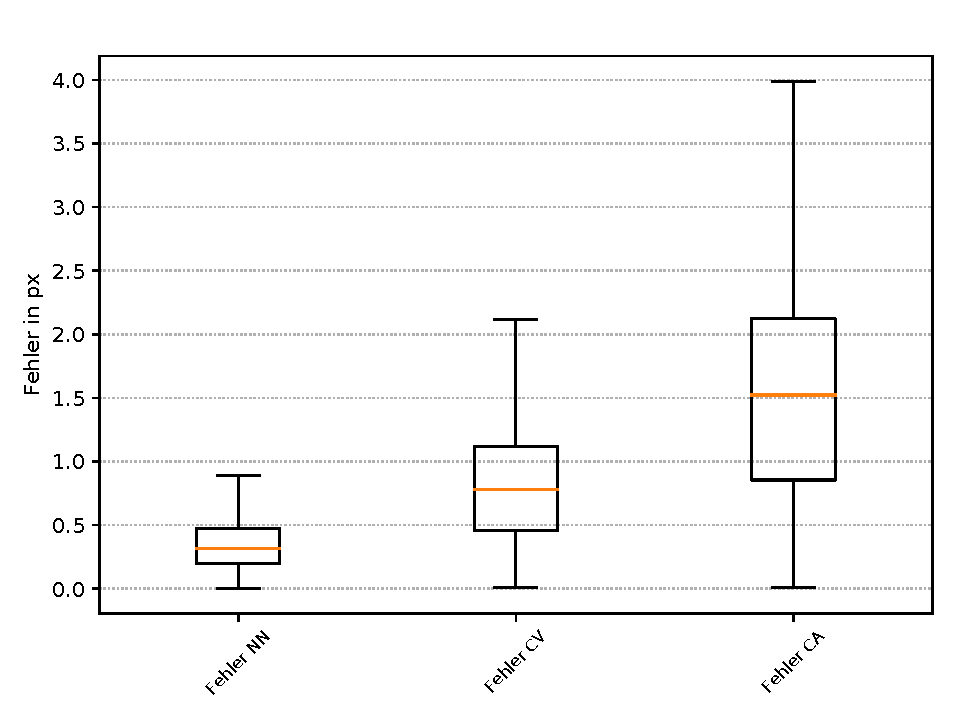
\includegraphics[width=0.8\textwidth]{appendix/RealSpheres-evaluation_NextStep_LocationError_2018-12-10_18-42-20.pdf}
    \caption{Boxplots für die NextStep-Ergebnisse Kugeln auf dem Förderband aus dem selbst aufgenommenen Datensatz.}
\end{figure}

\begin{figure}[h]
    \centering
	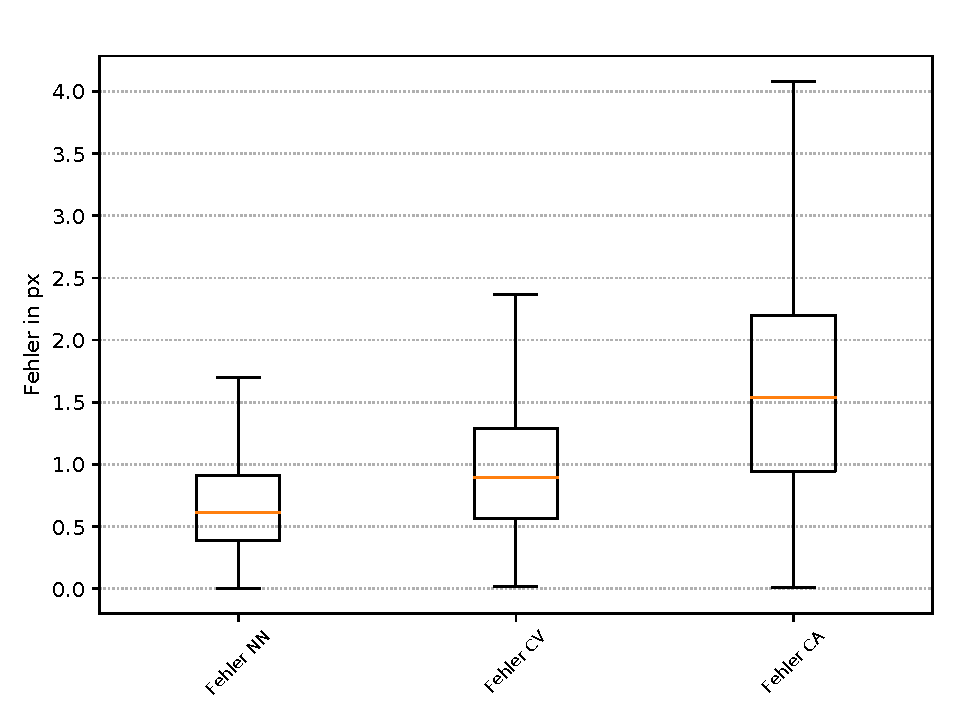
\includegraphics[width=0.8\textwidth]{appendix/RealPfeffer-evaluation_NextStep_LocationError_2018-12-10_18-43-24.pdf}
    \caption{Boxplots für die NextStep-Ergebnisse der Pfefferkörner auf dem Förderband aus dem selbst aufgenommenen Datensatz.}
\end{figure}

\begin{figure}[h]
    \centering
	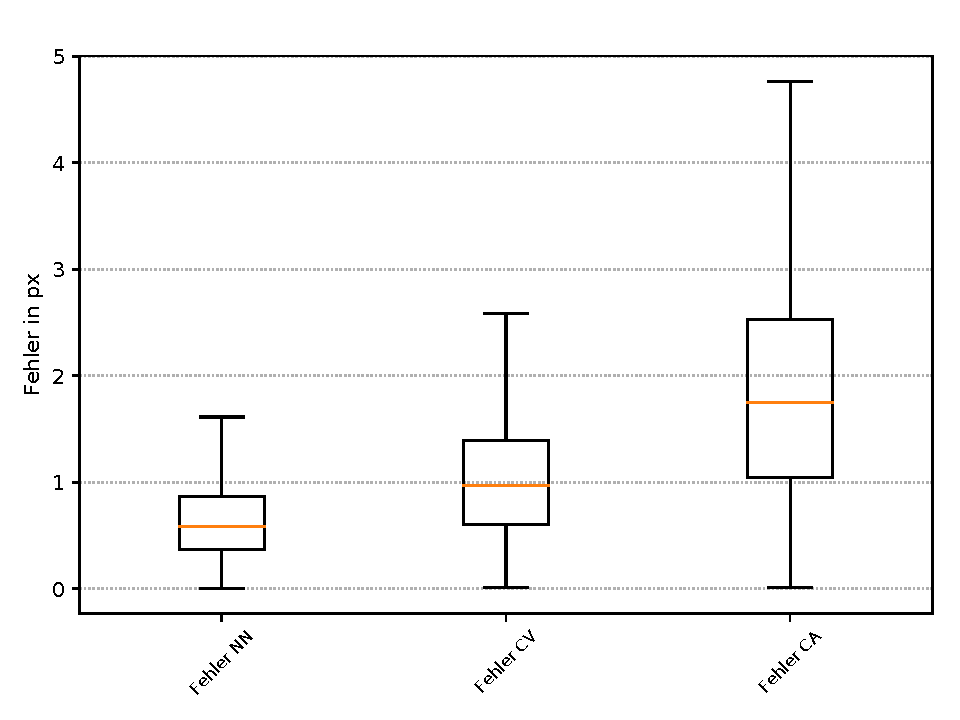
\includegraphics[width=0.8\textwidth]{appendix/RealZylinder-evaluation_NextStep_LocationError_2018-12-10_18-30-00.pdf}
    \caption{Boxplots für die NextStep-Ergebnisse der Zylinder auf dem Förderband aus dem selbst aufgenommenen Datensatz.}
\end{figure}

\begin{figure}[h]
    \centering
	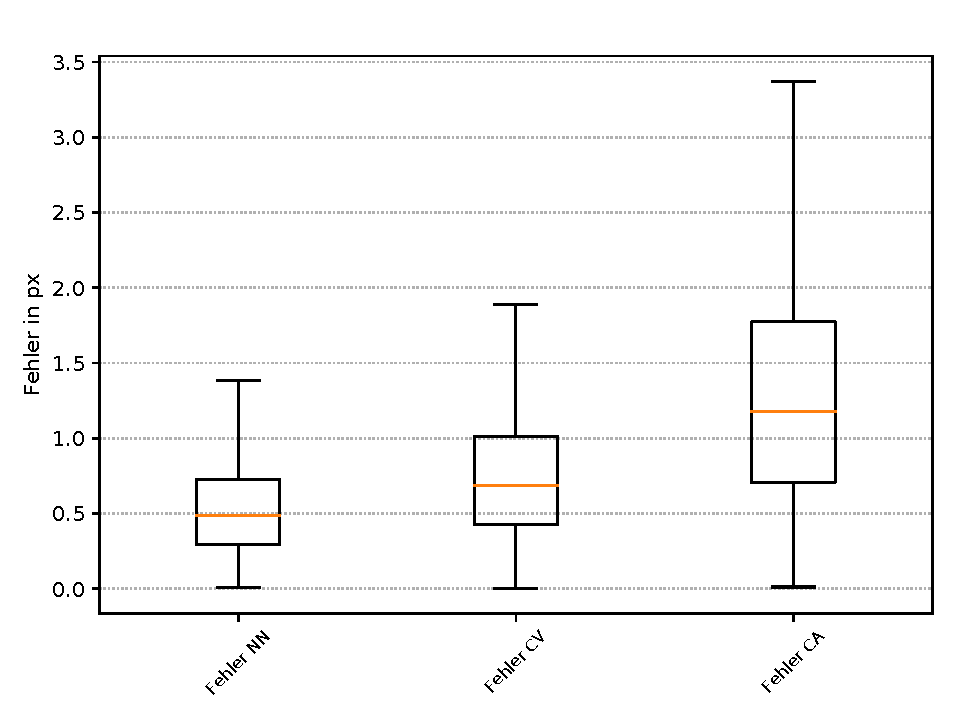
\includegraphics[width=0.8\textwidth]{appendix/RealWeizen-evaluation_NextStep_LocationError_2018-12-10_18-40-49.pdf}
    \caption{Boxplots für die NextStep-Ergebnisse der Zylinder auf dem Förderband aus dem selbst aufgenommenen Datensatz.}
\end{figure}

\begin{figure}[h]
    \centering
	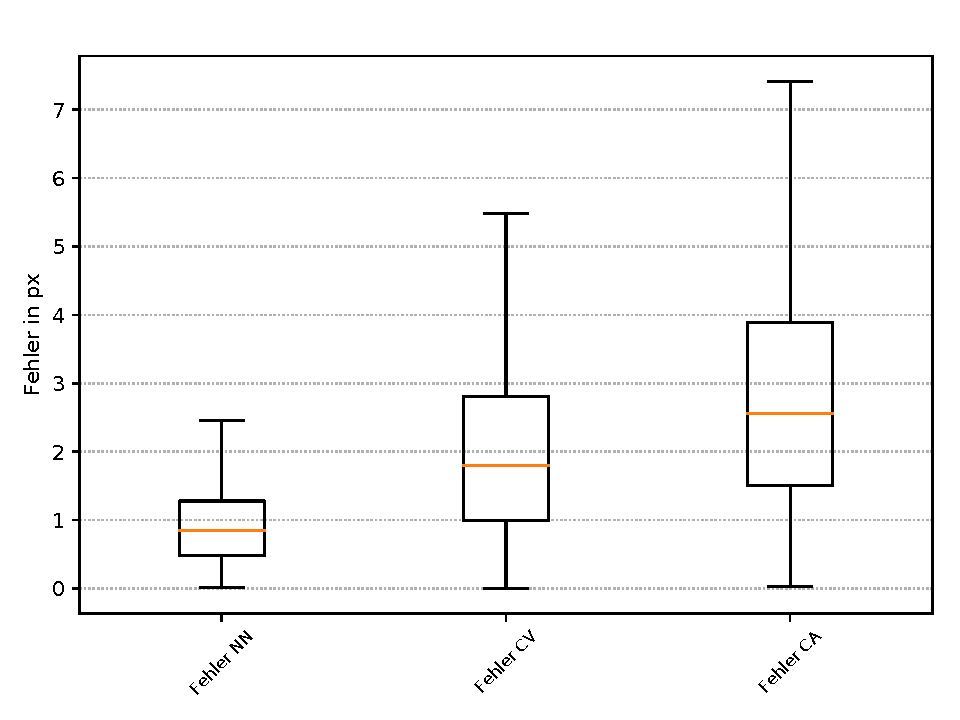
\includegraphics[width=0.8\textwidth]{appendix/RealSpheres-Rutsche-evaluation_NextStep_LocationError_2018-12-10_18-27-38.pdf}
    \caption{Boxplots für die NextStep-Ergebnisse der Kugeln auf der Rutsche aus dem selbst aufgenommenen Datensatz.}
\end{figure}

\begin{figure}[h]
    \centering
	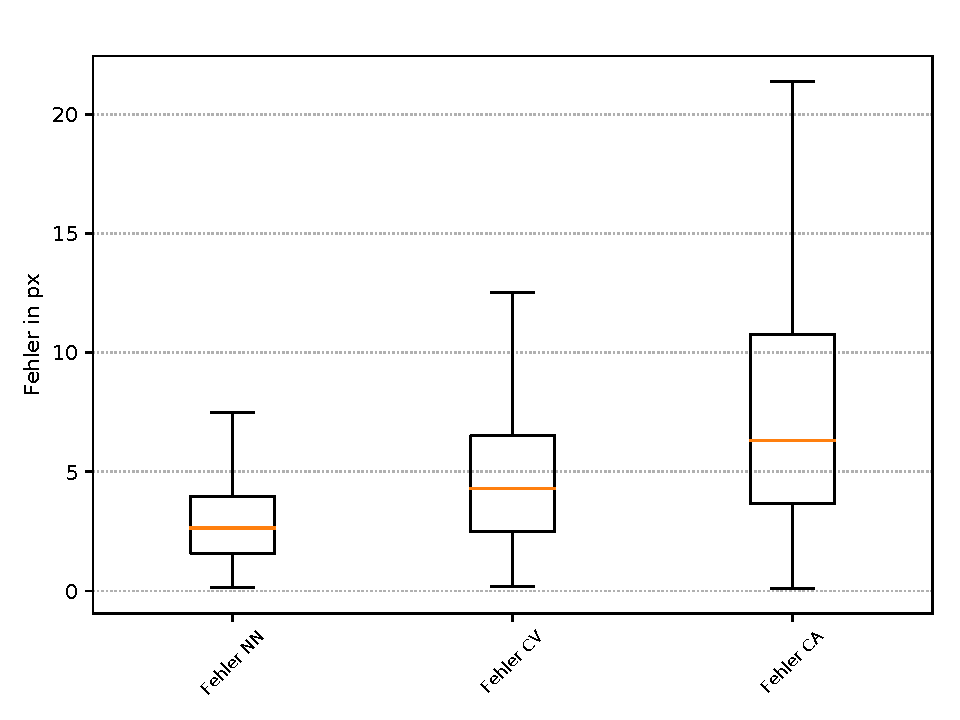
\includegraphics[width=0.8\textwidth]{appendix/RealPfeffer-Rutsche-evaluation_NextStep_LocationError_2018-12-10_18-28-28.pdf}
    \caption{Boxplots für die NextStep-Ergebnisse der Pfefferkörner auf der Rutsche aus dem selbst aufgenommenen Datensatz.}
\end{figure}

\begin{figure}[h]
    \centering
	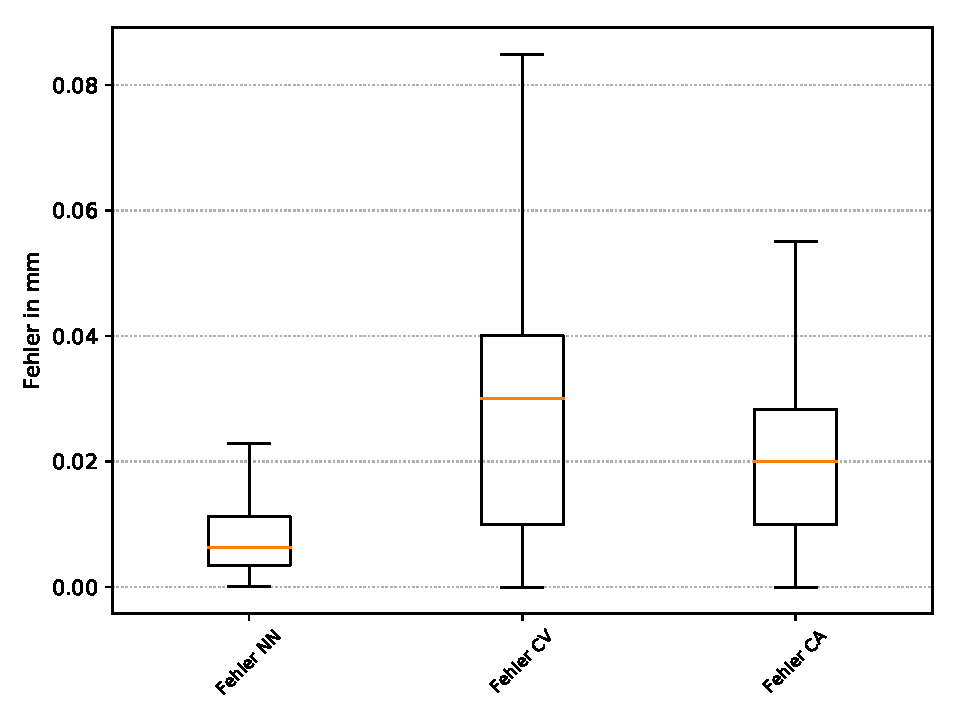
\includegraphics[width=0.8\textwidth]{appendix/SimulatedKugeln-evaluation_NextStep_LocationError_2018-12-17_15-28-43.pdf}
    \caption{Boxplots für die NextStep-Ergebnisse der Kugeln auf dem Förderband aus dem DEM-Datensatz.}
\end{figure}

\begin{figure}[h]
    \centering
	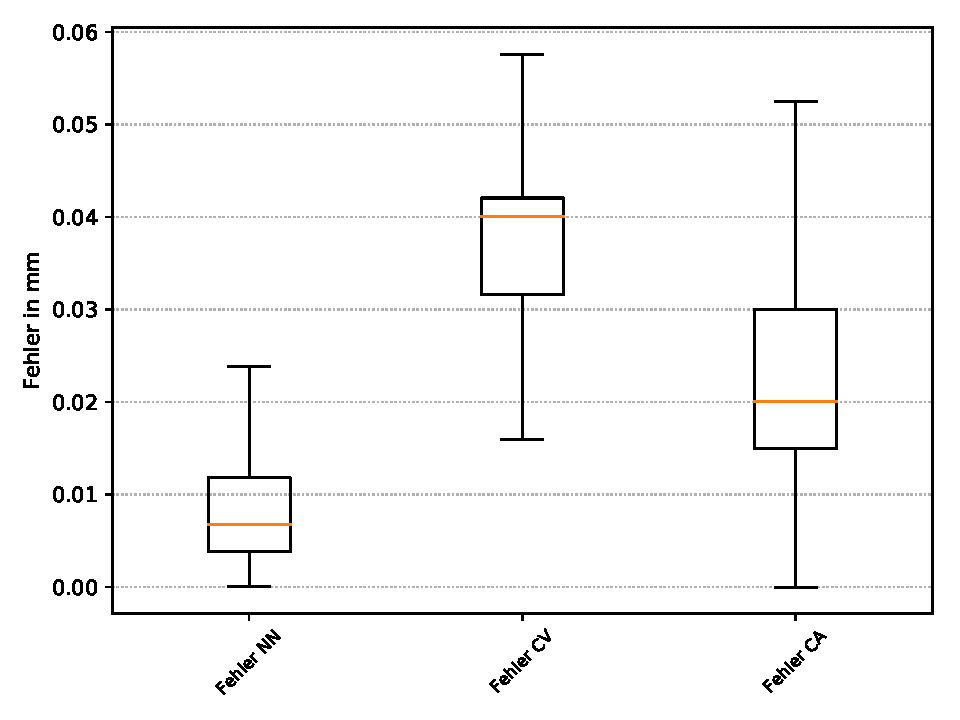
\includegraphics[width=0.8\textwidth]{appendix/SimCub-evaluation_NextStep_LocationError_2018-12-19_11-00-47.pdf}
    \caption{Boxplots für die NextStep-Ergebnisse der Plättchen auf dem Förderband aus dem DEM-Datensatz.}
\end{figure}



\begin{figure}[p]
    \centering
	% 
	\begin{subfigure}[t]{0.8\textwidth}
		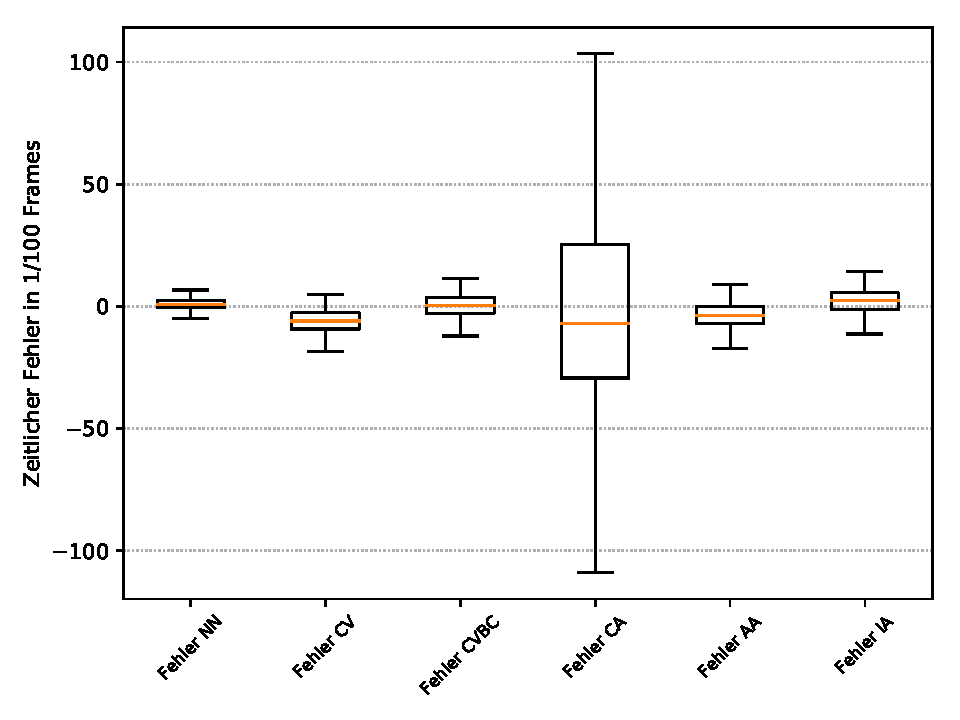
\includegraphics[width=\textwidth]{appendix/RealSpheres-evaluation_Separator_TimeErrorBoxplot_2018-12-11_14-05-52.pdf}
		\caption{Boxplots des zeitlichen Fehlers für die Separator-Ergebnisse der Kugeln aus dem selbst aufgenommenen Datensatz.}
		% \label{subfig:SimCubTimeBoxplot}
	\end{subfigure}
    % \quad
	\vskip\baselineskip
	
	\begin{subfigure}[t]{0.8\textwidth}
		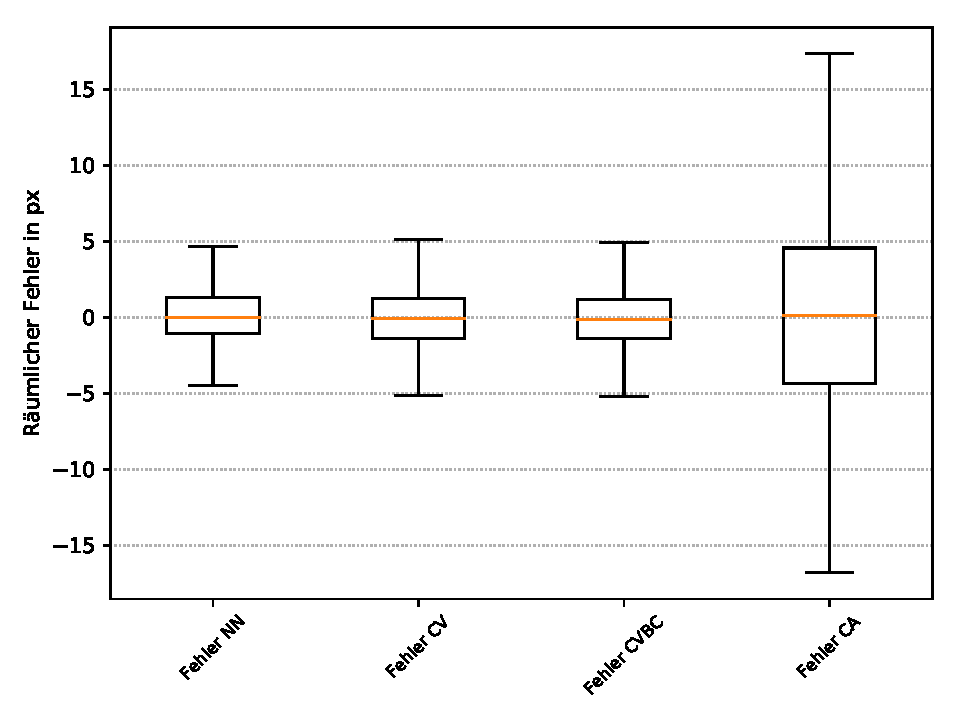
\includegraphics[width=\textwidth]{appendix/RealSpheres-evaluation_Separator_LocationErrorBoxplot_2018-12-11_14-05-52.pdf}
		\caption{Boxplots des örtlichen Fehlers für die Separator-Ergebnisse der Kugeln aus dem selbst aufgenommenen Datensatz.}
		% \label{subfig:SimCubLocBoxplot}
	\end{subfigure}
	
	\caption{Visualisierung der Ergebnisse für die Kugeln aus dem selbst aufgenommenen Datensatz.}
	% \label{fig:BoxplotsSimCub}
\end{figure}


\begin{figure}[p]
    \centering
	% 
	\begin{subfigure}[t]{0.8\textwidth}
		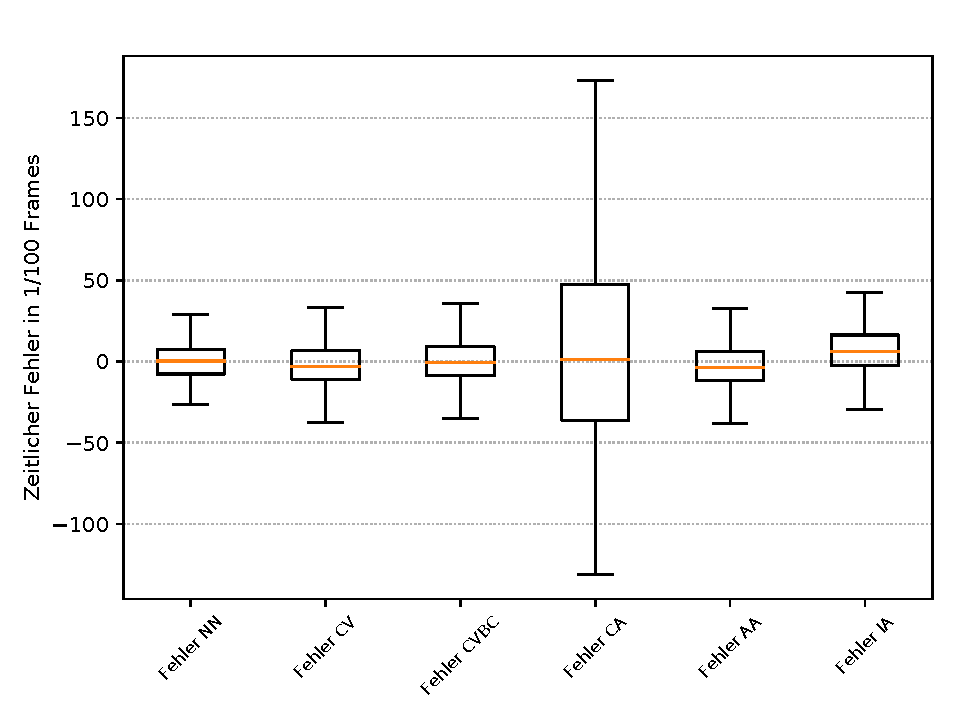
\includegraphics[width=\textwidth]{appendix/RealPfeffer-evaluation_Separator_TimeErrorBoxplot_2018-12-12_16-54-19.pdf}
		\caption{Boxplots des zeitlichen Fehlers für die Separator-Ergebnisse der Pfefferkörner aus dem selbst aufgenommenen Datensatz.}
		% \label{subfig:SimCubTimeBoxplot}
	\end{subfigure}
	% \quad
	\vskip\baselineskip
	
	\begin{subfigure}[t]{0.8\textwidth}
		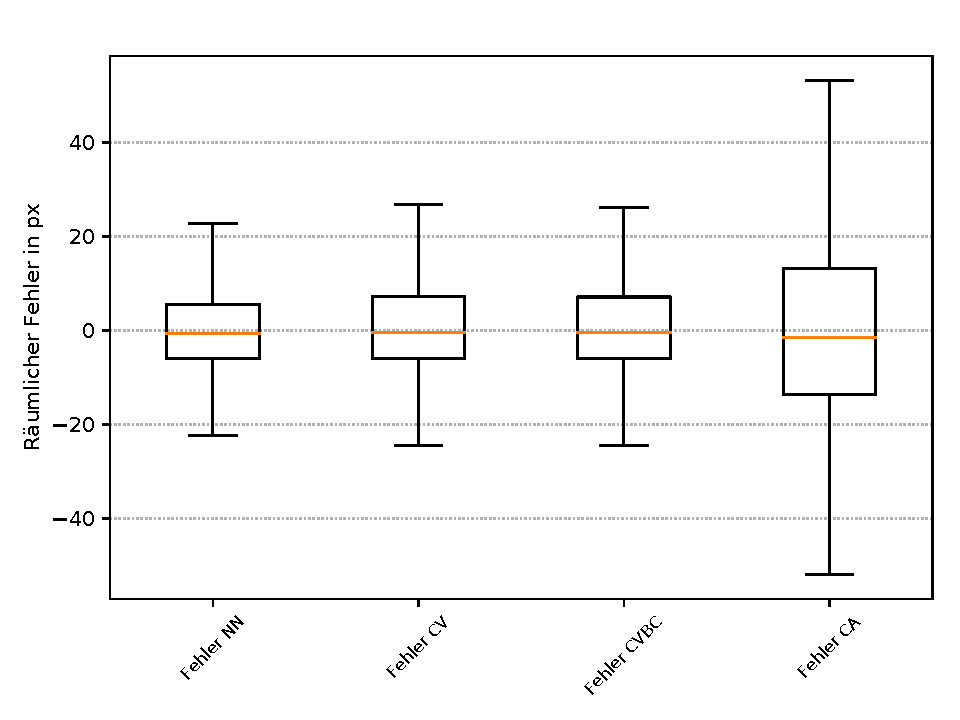
\includegraphics[width=\textwidth]{appendix/RealPfeffer-evaluation_Separator_LocationErrorBoxplot_2018-12-12_16-54-19.pdf}
		\caption{Boxplots des örtlichen Fehlers für die Separator-Ergebnisse der Pfefferkörner aus dem selbst aufgenommenen Datensatz.}
		% \label{subfig:SimCubLocBoxplot}
	\end{subfigure}
	
	\caption{Visualisierung der Ergebnisse für die Pfefferkörner aus dem selbst aufgenommenen Datensatz.}
	% \label{fig:BoxplotsSimCub}
\end{figure}


\begin{figure}[p]
    \centering
	% 
	\begin{subfigure}[t]{0.8\textwidth}
		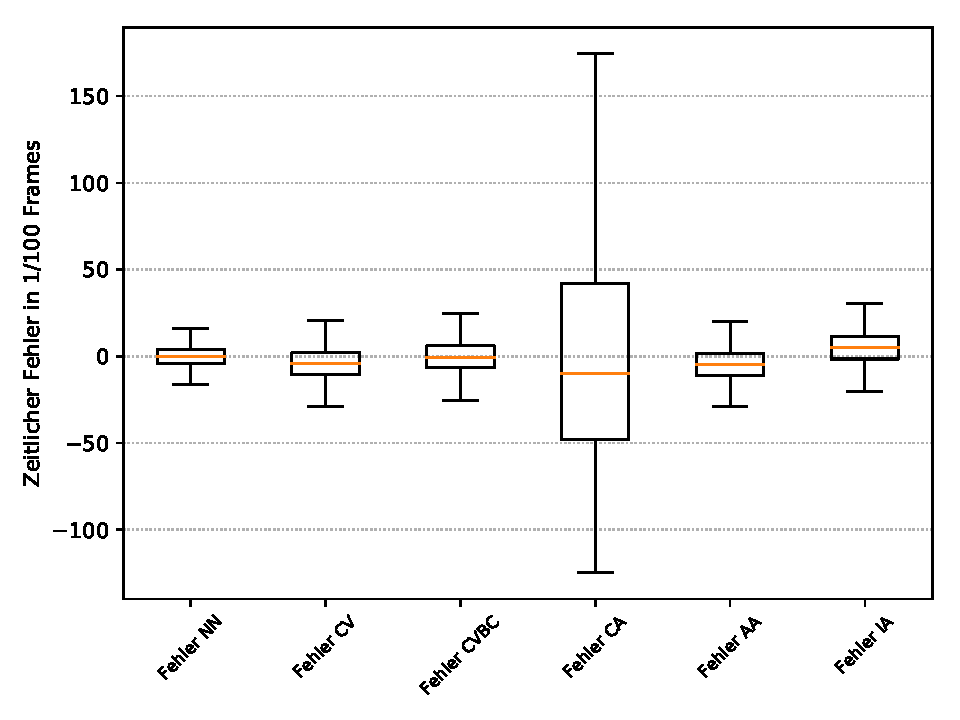
\includegraphics[width=\textwidth]{appendix/RealZylinder-evaluation_Separator_TimeErrorBoxplot_2018-12-11_14-11-28.pdf}
		\caption{Boxplots des zeitlichen Fehlers für die Separator-Ergebnisse der Zylinder aus dem selbst aufgenommenen Datensatz.}
		% \label{subfig:SimCubTimeBoxplot}
	\end{subfigure}
    % \quad
	\vskip\baselineskip
	
	\begin{subfigure}[t]{0.8\textwidth}
		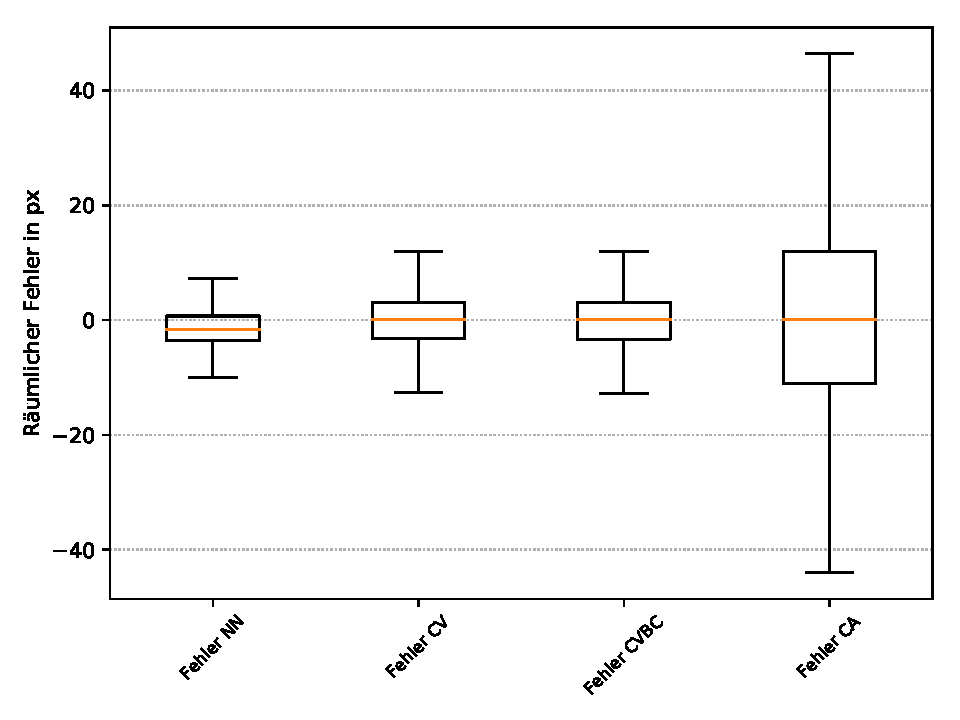
\includegraphics[width=\textwidth]{appendix/RealZylinder-evaluation_Separator_LocationErrorBoxplot_2018-12-11_14-11-28.pdf}
		\caption{Boxplots des örtlichen Fehlers für die Separator-Ergebnisse der Zylinder aus dem selbst aufgenommenen Datensatz.}
		% \label{subfig:SimCubLocBoxplot}
	\end{subfigure}
	
	\caption{Visualisierung der Ergebnisse für die Zylinder aus dem selbst aufgenommenen Datensatz.}
	% \label{fig:BoxplotsSimCub}
\end{figure}

\begin{figure}[p]
    \centering
	% 
	\begin{subfigure}[t]{0.8\textwidth}
		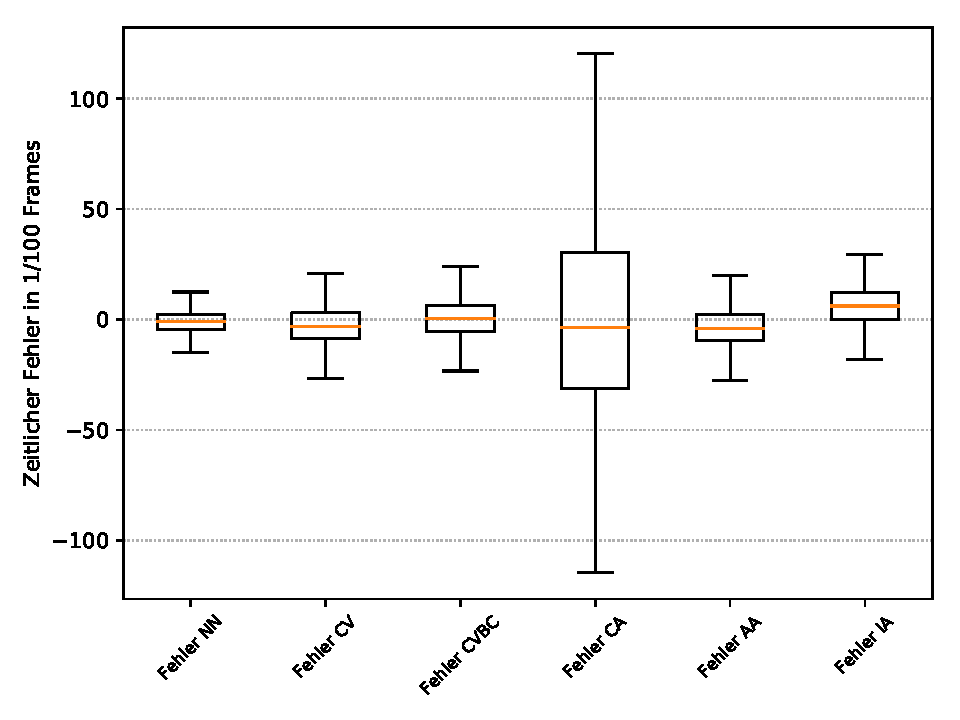
\includegraphics[width=\textwidth]{appendix/RealWeizen-evaluation_Separator_TimeErrorBoxplot_2018-12-11_14-09-12.pdf}
		\caption{Boxplots des zeitlichen Fehlers für die Separator-Ergebnisse der Weizenkörner aus dem selbst aufgenommenen Datensatz.}
		% \label{subfig:SimCubTimeBoxplot}
	\end{subfigure}
    % \quad
	\vskip\baselineskip
	
	\begin{subfigure}[t]{0.8\textwidth}
		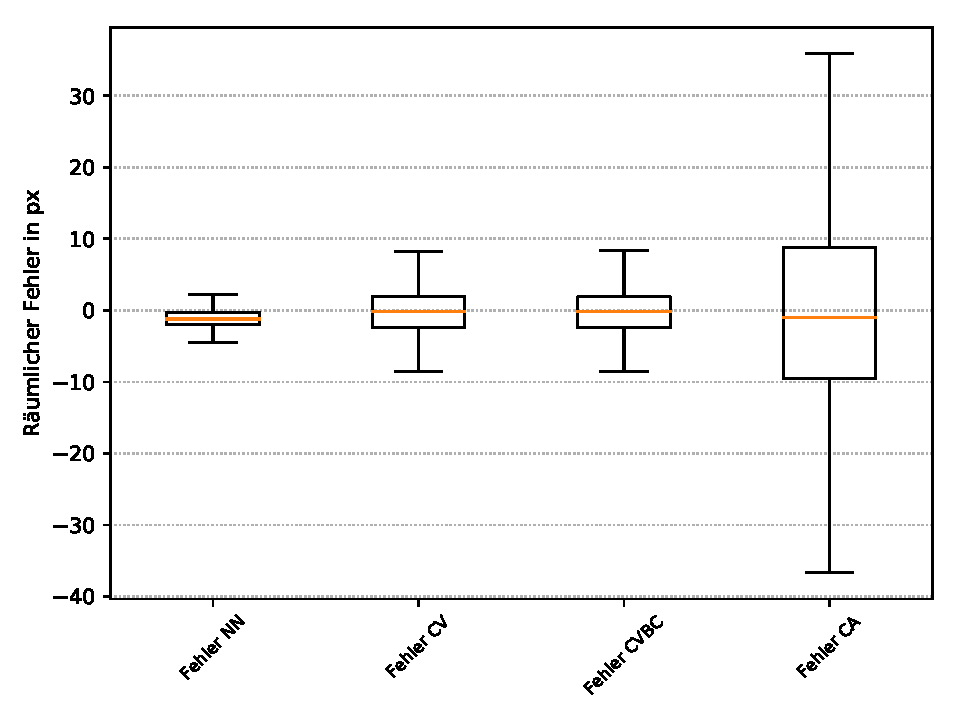
\includegraphics[width=\textwidth]{appendix/RealWeizen-evaluation_Separator_LocationErrorBoxplot_2018-12-11_14-09-12.pdf}
		\caption{Boxplots des örtlichen Fehlers für die Separator-Ergebnisse der Weizenkörner aus dem selbst aufgenommenen Datensatz.}
		% \label{subfig:SimCubLocBoxplot}
	\end{subfigure}
	
	\caption{Visualisierung der Ergebnisse für die Weizenkörner aus dem selbst aufgenommenen Datensatz.}
	% \label{fig:BoxplotsSimCub}
\end{figure}

\begin{figure}[p]
    \centering
	% 
	\begin{subfigure}[t]{0.8\textwidth}
		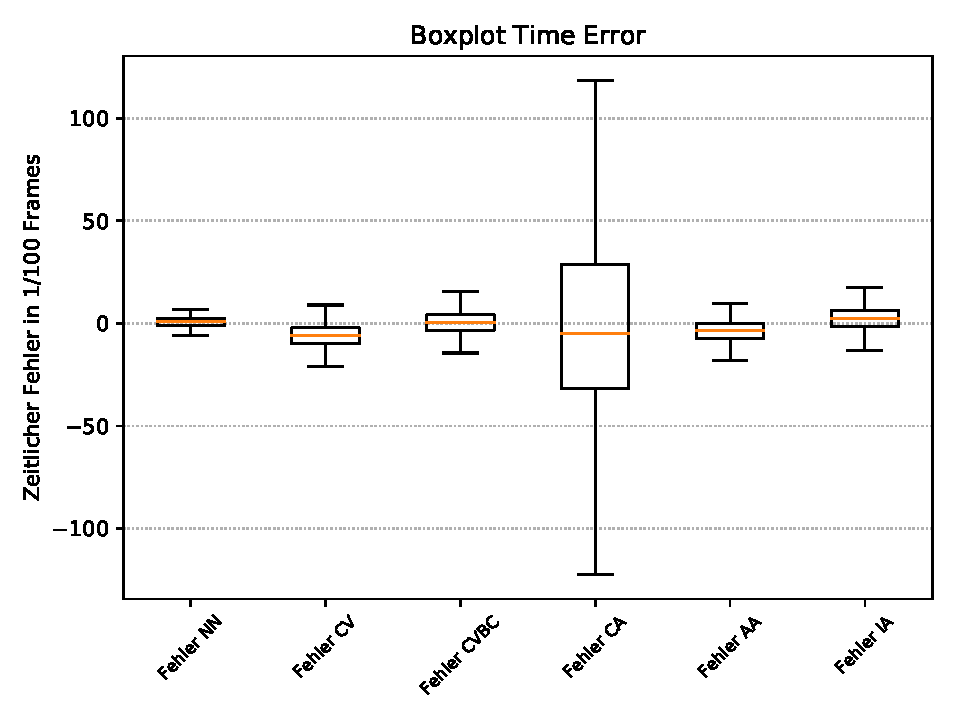
\includegraphics[width=\textwidth]{appendix/RealSpheres_Rutsche-evaluation_Separator_TimeErrorBoxplot_2018-12-08_10-45-13.pdf}
		\caption{Boxplots des zeitlichen Fehlers für die Separator-Ergebnisse der Kugeln auf der Rutsche aus dem selbst aufgenommenen Datensatz.}
		% \label{subfig:SimCubTimeBoxplot}
	\end{subfigure}
    % \quad
	\vskip\baselineskip
	
	\begin{subfigure}[t]{0.8\textwidth}
		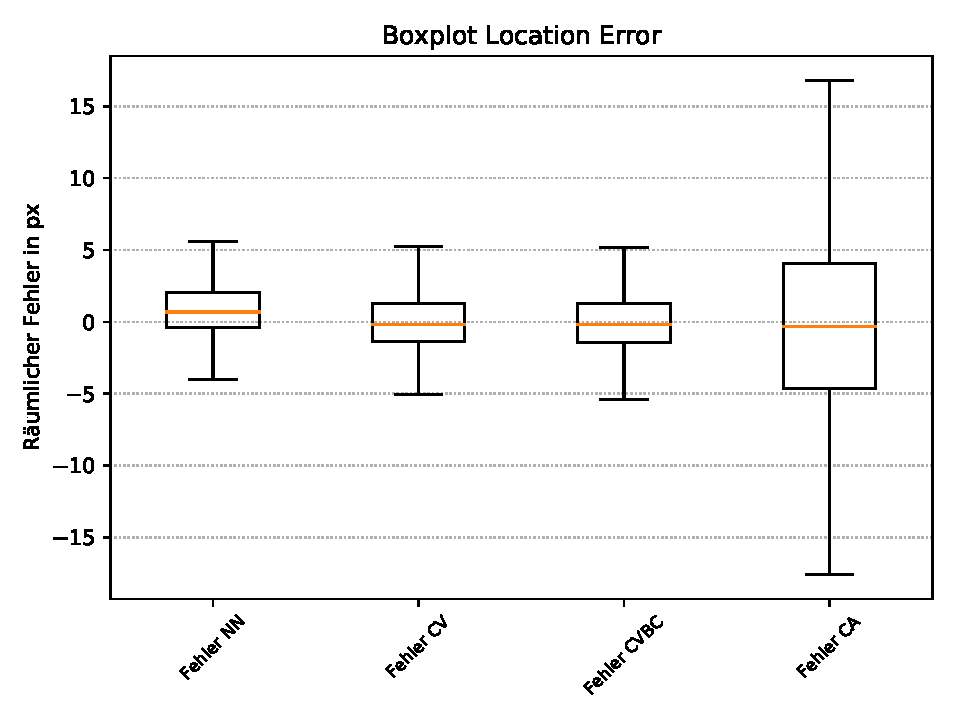
\includegraphics[width=\textwidth]{appendix/RealSpheres_Rutsche-evaluation_Separator_LocationErrorBoxplot_2018-12-08_10-45-13.pdf}
		\caption{Boxplots des örtlichen Fehlers für die Separator-Ergebnisse der Kugeln auf der Rutsche aus dem selbst aufgenommenen Datensatz.}
		% \label{subfig:SimCubLocBoxplot}
	\end{subfigure}
	
	\caption{Visualisierung der Ergebnisse für die Kugeln auf der Rutsche aus dem selbst aufgenommenen Datensatz.}
	% \label{fig:BoxplotsSimCub}
\end{figure}

\begin{figure}[p]
    \centering
	% 
	\begin{subfigure}[t]{0.8\textwidth}
		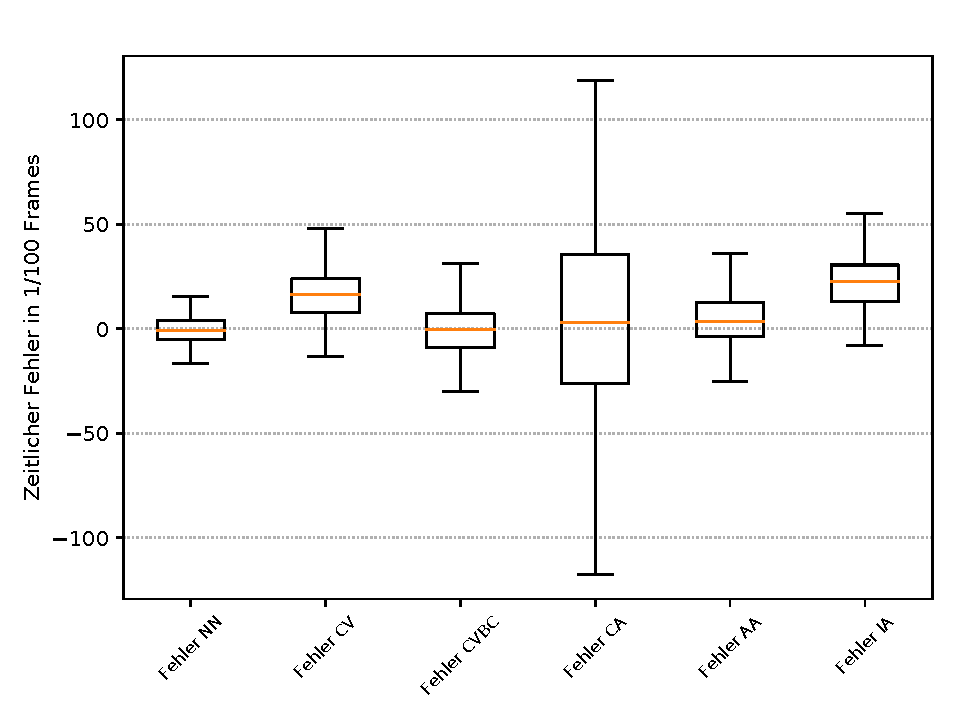
\includegraphics[width=\textwidth]{appendix/RealPfeffer_Rutsche-evaluation_Separator_TimeErrorBoxplot_2018-12-13_13-49-57.pdf}
		\caption{Boxplots des zeitlichen Fehlers für die Separator-Ergebnisse der Pfefferkörner auf der Rutsche aus dem selbst aufgenommenen Datensatz.}
		% \label{subfig:SimCubTimeBoxplot}
	\end{subfigure}
    % \quad
	\vskip\baselineskip
	
	\begin{subfigure}[t]{0.8\textwidth}
		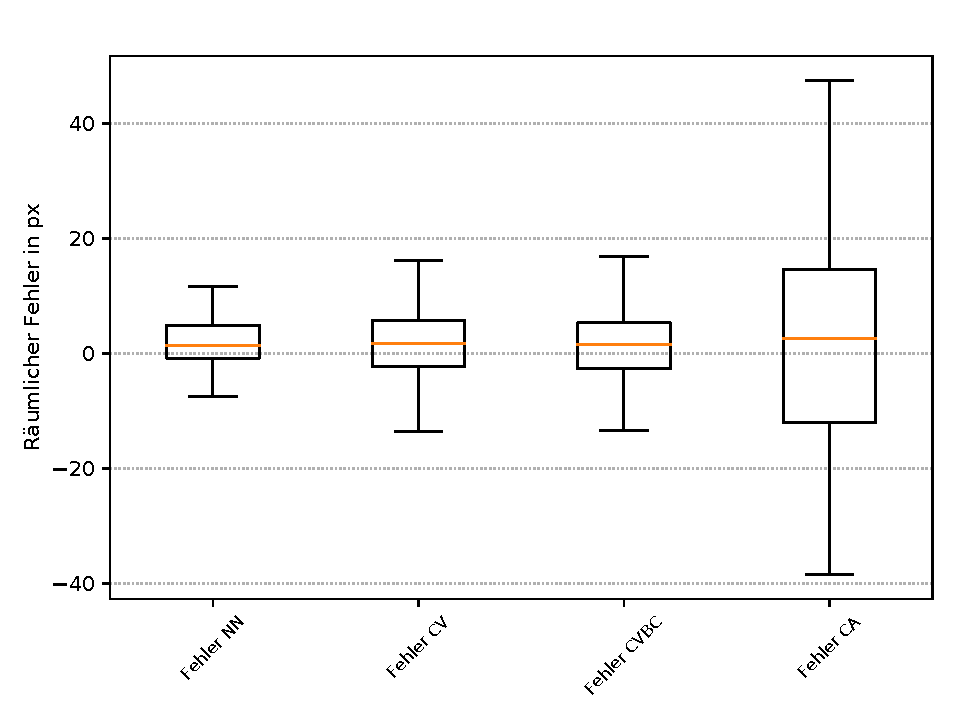
\includegraphics[width=\textwidth]{appendix/RealPfeffer_Rutsche-evaluation_Separator_LocationErrorBoxplot_2018-12-13_13-49-57.pdf}
		\caption{Boxplots des örtlichen Fehlers für die Separator-Ergebnisse der Pfefferkörner auf der Rutsche aus dem selbst aufgenommenen Datensatz.}
		% \label{subfig:SimCubLocBoxplot}
	\end{subfigure}
	
	\caption{Visualisierung der Ergebnisse für die Pfefferkörner auf der Rutsche aus dem selbst aufgenommenen Datensatz.}
	% \label{fig:BoxplotsSimCub}
\end{figure}

\begin{figure}[p]
    \centering
	% 
	\begin{subfigure}[t]{0.8\textwidth}
		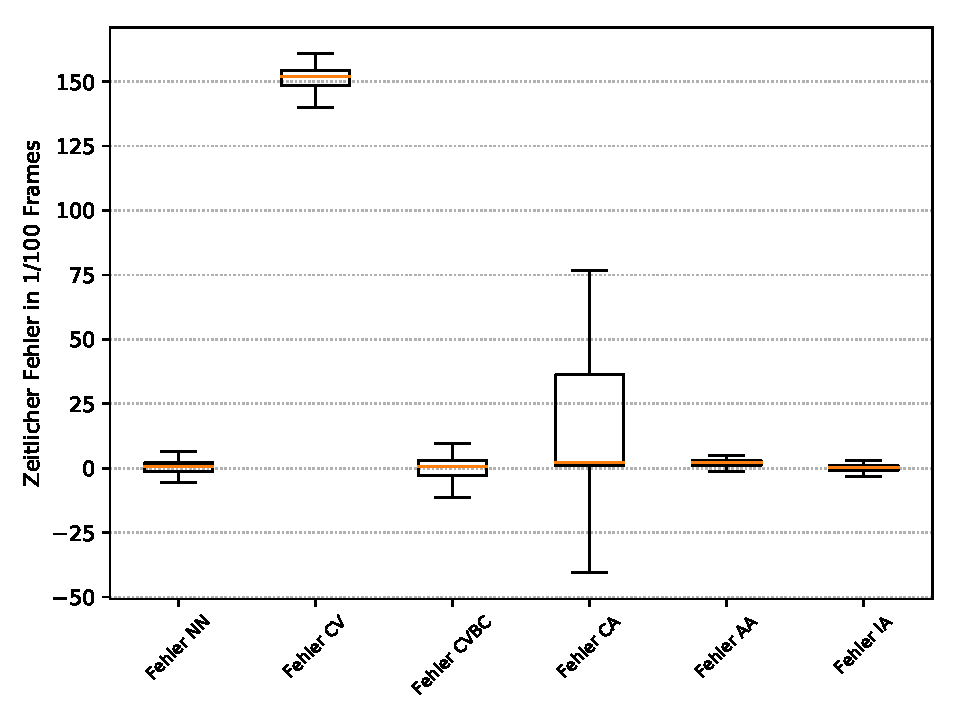
\includegraphics[width=\textwidth]{appendix/SimSpheres-evaluation_Separator_TimeErrorBoxplot_2018-12-11_14-27-07.pdf}
		\caption{Boxplots des zeitlichen Fehlers für die Separator-Ergebnisse der Kugeln aus dem DEM-Datensatz.}
		% \label{subfig:SimCubTimeBoxplot}
	\end{subfigure}
    % \quad
	\vskip\baselineskip
	
	\begin{subfigure}[t]{0.8\textwidth}
		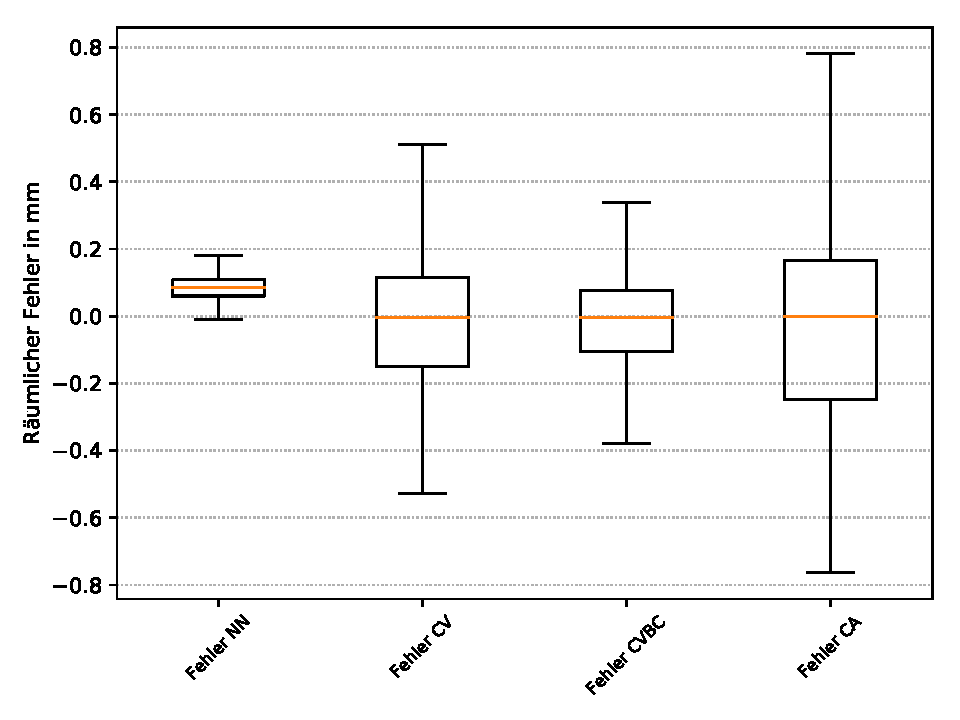
\includegraphics[width=\textwidth]{appendix/SimSpheres-evaluation_Separator_LocationErrorBoxplot_2018-12-11_14-27-07.pdf}
		\caption{Boxplots des örtlichen Fehlers für die Separator-Ergebnisse der Kugeln aus dem DEM-Datensatz.}
		% \label{subfig:SimCubLocBoxplot}
	\end{subfigure}
	
	\caption{Visualisierung der Ergebnisse für die Kugeln aus der DEM-Simulation.}
	% \label{fig:BoxplotsSimCub}
\end{figure}

\begin{figure}[p]
    \centering
	% 
	\begin{subfigure}[t]{0.8\textwidth}
		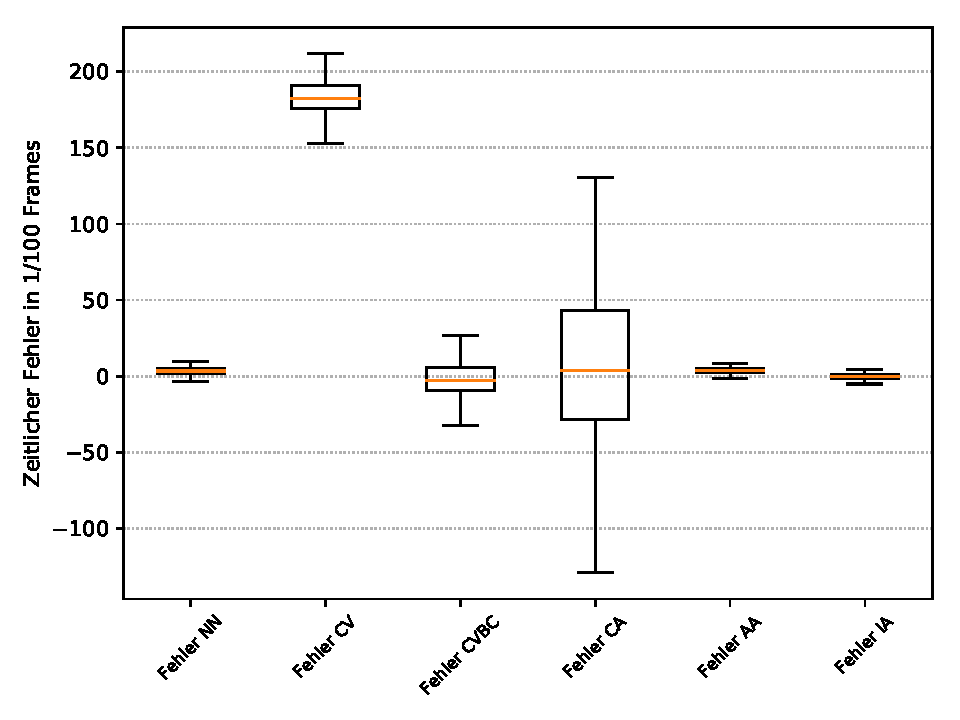
\includegraphics[width=\textwidth]{appendix/SimCub-evaluation_Separator_TimeErrorBoxplot_2018-12-11_14-33-22.pdf}
		\caption{Boxplots des zeitlichen Fehlers für die Separator-Ergebnisse der Plättchen aus dem DEM-Datensatz.}
		% \label{subfig:SimCubTimeBoxplot}
	\end{subfigure}
    % \quad
	\vskip\baselineskip
	
	\begin{subfigure}[t]{0.8\textwidth}
		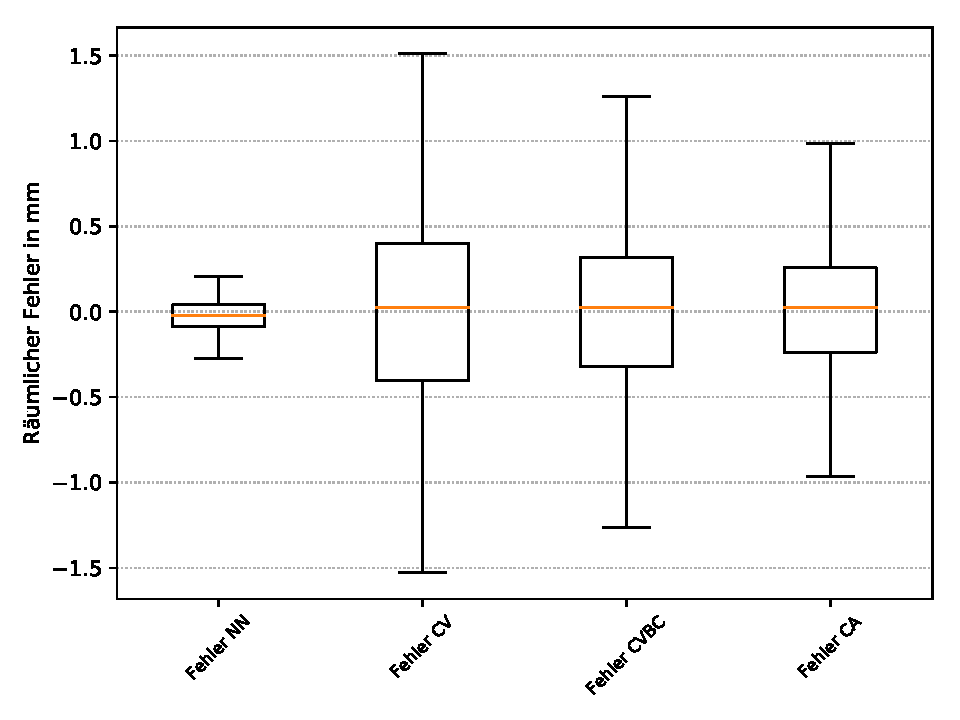
\includegraphics[width=\textwidth]{appendix/SimCub-evaluation_Separator_LocationErrorBoxplot_2018-12-11_14-33-22.pdf}
		\caption{Boxplots des örtlichen Fehlers für die Separator-Ergebnisse der Plättchen aus dem DEM-Datensatz.}
		% \label{subfig:SimCubLocBoxplot}
	\end{subfigure}
	
	\caption{Visualisierung der Ergebnisse für die Plättchen aus der DEM-Simulation.}
	% \label{fig:BoxplotsSimCub}
\end{figure}


% \begin{adjustbox}{angle=90}
    % \begin{tabular}{lrrrrrrrrrrrrrrrr}
    %     \toprule
    %     {} &      X\_0 &      X\_1 &      X\_2 &      X\_3 &      X\_4 &      X\_5 &      X\_6 &       Y\_0 &       Y\_1 &       Y\_2 &       Y\_3 &       Y\_4 &       Y\_5 &       Y\_6 &  LabelPosBalken &  LabelTime \\
    %     \midrule
    %     97943 &  0.51419 &  0.52039 &  0.52663 &  0.53290 &  0.53922 &  0.54558 &  0.55197 &  0.071913 &  0.071879 &  0.071846 &  0.071813 &  0.071779 &  0.071746 &  0.071713 &        0.071069 &  21.653686 \\
    %     88546 &  0.51393 &  0.52011 &  0.52632 &  0.53257 &  0.53887 &  0.54520 &  0.55157 &  0.111160 &  0.111100 &  0.111030 &  0.110970 &  0.110910 &  0.110840 &  0.110780 &        0.109549 &  21.785216 \\
    %     16959 &  0.51271 &  0.51886 &  0.52506 &  0.53129 &  0.53756 &  0.54387 &  0.55022 &  0.103270 &  0.103270 &  0.103280 &  0.103280 &  0.103280 &  0.103280 &  0.103280 &        0.103320 &  22.034965 \\
    %     70961 &  0.51780 &  0.52393 &  0.53009 &  0.53630 &  0.54255 &  0.54883 &  0.55515 &  0.141970 &  0.141940 &  0.141910 &  0.141890 &  0.141860 &  0.141840 &  0.141810 &        0.141326 &  21.433004 \\
    %     64163 &  0.51326 &  0.51943 &  0.52564 &  0.53190 &  0.53819 &  0.54452 &  0.55089 &  0.059104 &  0.059104 &  0.059105 &  0.059106 &  0.059107 &  0.059108 &  0.059108 &        0.059124 &  21.885475 \\
    %     \bottomrule
    %     \end{tabular}
    
%     \begin{table}

%         \begin{subtable}{1\textwidth}
%         \sisetup{table-format=-1.2}   % 2 decimals, leave space for minus sign
%         \centering

%     \begin{tabular}{lrrrrrrrrrrrrrr}
%         \toprule
%         {} &      X\_0 &      X\_1 &      X\_2 &      X\_3 &      X\_4 &      X\_5 &      X\_6 &       Y\_0 &       Y\_1 &       Y\_2 &       Y\_3 &       Y\_4 &       Y\_5 &       Y\_6 \\
%         \midrule
%         24047  &  0.51383 &  0.51980 &  0.52580 &  0.53185 &  0.53794 &  0.54406 &  0.55023 &  0.128630 &  0.128630 &  0.128630 &  0.128640 &  0.128640 &  0.128640 &  0.128640 \\
%         123713 &  0.51261 &  0.51876 &  0.52495 &  0.53118 &  0.53745 &  0.54376 &  0.55011 &  0.056767 &  0.056682 &  0.056597 &  0.056513 &  0.056428 &  0.056344 &  0.056259 \\
%         65266  &  0.51846 &  0.52462 &  0.53081 &  0.53704 &  0.54332 &  0.54963 &  0.55598 &  0.072922 &  0.073136 &  0.073349 &  0.073563 &  0.073775 &  0.073988 &  0.074200 \\
%         97314  &  0.51319 &  0.51936 &  0.52557 &  0.53182 &  0.53810 &  0.54443 &  0.55079 &  0.130030 &  0.130030 &  0.130030 &  0.130030 &  0.130040 &  0.130040 &  0.130040 \\
%         102086 &  0.51812 &  0.52422 &  0.53035 &  0.53653 &  0.54275 &  0.54900 &  0.55530 &  0.082149 &  0.082076 &  0.082004 &  0.081931 &  0.081859 &  0.081786 &  0.081714 \\
%         \bottomrule
%     \end{tabular}

%     \caption{First subtable}\label{tab:sub_first}
%     \end{subtable}
    
%     \bigskip
% \begin{subtable}{1\textwidth}
% \sisetup{table-format=4.0} % integer values only, up to 4 digits
% \centering
    
%     \begin{tabular}{lrrrr}
%         \toprule
%         {} &  LabelPosBalken &  LabelTime &  NNPredictionPosBalken &  NNPredictionTime \\
%         \midrule
%         24047  &        0.128680 &  22.622669 &               0.128833 &         22.592078 \\
%         123713 &        0.054585 &  22.055866 &               0.054541 &         22.047100 \\
%         65266  &        0.078287 &  21.237360 &               0.078345 &         21.232997 \\
%         97314  &        0.130050 &  21.907821 &               0.130058 &         21.901709 \\
%         102086 &        0.080331 &  21.498588 &               0.080367 &         21.508065 \\
%         \bottomrule
%     \end{tabular}

%     \caption{Second subtable}\label{tab:sub_second}
% \end{subtable}

% \bigskip
% \begin{subtable}{1\textwidth}
% \sisetup{table-format=1.2} % up to two decimal digits, no minus signs
% \centering
    
%     \begin{tabular}{lrrrrrrrrr}
%         \toprule
%         {} &  CV\_Prediction\_Time &  CVBC\_Prediction\_Loc &  CVBC\_Prediction\_Time &  CA\_Prediction\_Loc &  CA\_Prediction\_Time &  AA\_Prediction\_Loc &  AA\_Prediction\_Time &  IA\_Prediction\_Loc &  IA\_Prediction\_Time \\
%         \midrule
%         24047  &           24.273906 &             0.128640 &             22.760258 &           0.128640 &           22.265233 &           0.128640 &           22.615945 &           0.128640 &           22.595541 \\
%         123713 &           23.604724 &             0.054381 &             22.091076 &           0.054139 &           22.070526 &           0.054139 &           22.070526 &           0.054141 &           22.051517 \\
%         65266  &           22.680315 &             0.078687 &             21.166667 &           0.078481 &           21.257118 &           0.078481 &           21.257118 &           0.078477 &           21.239404 \\
%         97314  &           23.460692 &             0.130040 &             21.947044 &           0.130040 &           22.288995 &           0.130040 &           21.946125 &           0.130040 &           21.927343 \\
%         102086 &           22.968254 &             0.080169 &             21.454606 &           0.080413 &           21.186956 &           0.080397 &           21.500698 &           0.080398 &           21.482475 \\
%         \bottomrule
%     \end{tabular}

%     asdasdd \\

%     \begin{tabular}{lrrrrrrrrrrrr}
%         \toprule
%         {} &  NNpixelErrorPosBalken &  NNerrorTime &  CVpixelErrorPosBalken &  CVerrorTime &  CVBCpixelErrorPosBalken &  CVBCerrorTime &  CApixelErrorPosBalken &  CAerrorTime &  AApixelErrorPosBalken &  AAerrorTime &  IApixelErrorPosBalken &  IAerrorTime \\
%         \midrule
%         24047  &               0.000153 &    -0.030590 &              -0.000040 &     1.651237 &                -0.000040 &       0.137589 &              -0.000040 &    -0.357436 &              -0.000040 &    -0.006724 &              -0.000040 &    -0.027128 \\
%         123713 &              -0.000044 &    -0.008766 &              -0.000332 &     1.548858 &                -0.000204 &       0.035211 &              -0.000446 &     0.014660 &              -0.000446 &     0.014660 &              -0.000444 &    -0.004349 \\
%         65266  &               0.000058 &    -0.004362 &               0.000721 &     1.442955 &                 0.000400 &      -0.070693 &               0.000194 &     0.019758 &               0.000194 &     0.019758 &               0.000190 &     0.002045 \\
%         97314  &               0.000008 &    -0.006113 &              -0.000010 &     1.552871 &                -0.000010 &       0.039223 &              -0.000010 &     0.381174 &              -0.000010 &     0.038303 &              -0.000010 &     0.019522 \\
%         102086 &               0.000036 &     0.009478 &              -0.000270 &     1.469666 &                -0.000161 &      -0.043982 &               0.000082 &    -0.311632 &               0.000067 &     0.002111 &               0.000067 &    -0.016113 \\
%         \bottomrule
%     \end{tabular}
      
%     \caption{Third subtable}\label{tab:sub_third}
% \end{subtable}

% \caption{Three simple tables} \label{tab:three_tables}
% \end{table}
    

% \end{adjustbox}